\renewcommand{\FileName}{loginfl}
\begin{frame}
  \frametitle{Influence measures and diagnostic plots}
  \begin{itemize}
	\item{\large\bfseries Leverage}: Potential impact of an individual case $\sim$ distance
	from the centroid in space of predictors
	\item{\large\bfseries Residuals}: Which observations are poorly fitted? 
	\item{\large\bfseries Influence}: Actual impact of an individual case $\sim$ leverage $\times$ residual
      \begin{itemize*}
	  \item \boldital{C}, \boldital{CBAR} -- analogs of Cook's D in OLS $\sim$ standardized change in
	  regression coefficients when $i$-th case is deleted.
		\item \boldital{DIFCHISQ}, \boldital{DIFDEV} -- $\Delta \chi^2$ when $i$-th case is deleted.
	  \end{itemize*}
  \end{itemize}
 \begin{center}
  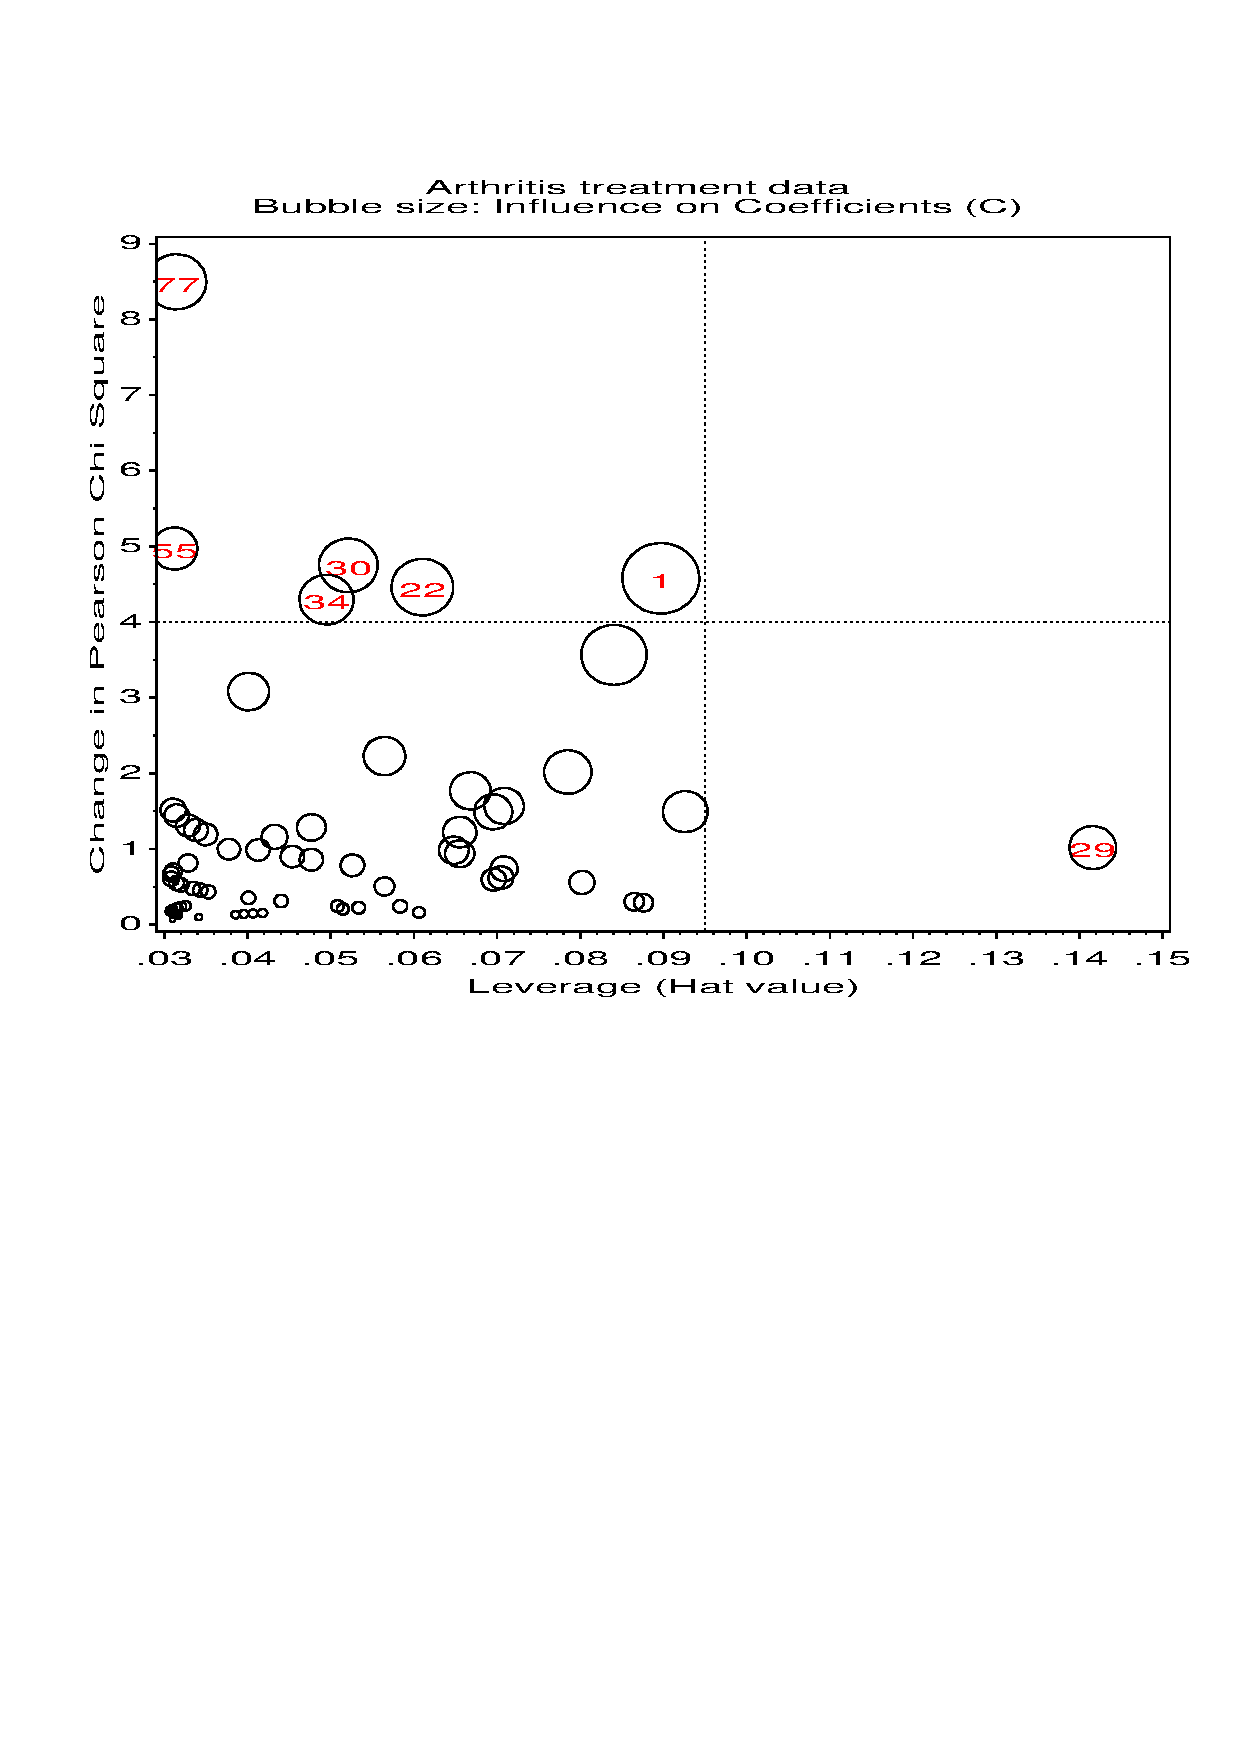
\includegraphics[width=.4\dispwidth,clip]{fig/logist1b2}
 \end{center}
\end{frame}

\begin{frame}[fragile,allowframebreaks]
  \frametitle{Influence measures and diagnostic plots}
\PROC{LOGISTIC}: printed output with the \texttt{influence} and \texttt{iplots} options
\begin{Input}
proc logistic data=arthrit ;
   model better = sex treat age / \sasemph{influence iplots};
\end{Input}

\begin{Output}[fontsize=\footnotesize,baselinestretch=0.6]
                     The LOGISTIC Procedure
                     Regression Diagnostics
          Deviance Residual               Hat Matrix Diagonal

Case             (1 unit = 0.26)               (1 unit = 0.01)
Number  Value   -8  -4  0 2 4 6 8     Value   0 2 4 6 8  12  16

   1    1.812  | *      |        |    0.089  |          *      |
   2    0.360  |        |*       |    0.031  |    *            |
   3    0.685  |        |  *     |    0.087  |          *      |
   4    0.425  |        | *      |    0.034  |    *            |
   5    0.700  |        |  *     |    0.086  |          *      |
   6    0.488  |        | *      |    0.038  |    *            |
   7    1.703  |  *     |        |    0.084  |         *       |
   8    0.499  |        | *      |    0.039  |    *            |
   9    1.396  |   *    |        |    0.066  |        *        |
  10    0.511  |        | *      |    0.040  |     *           |
  11    1.142  |    *   |        |    0.064  |       *         |
  12    0.523  |        | *      |    0.041  |     *           |
  13    1.234  |        |    *   |    0.065  |       *         |
  14    0.599  |        | *      |    0.051  |      *          |
  15    1.121  |    *   |        |    0.065  |       *         |
  16    0.599  |        | *      |    0.051  |      *          |
  17    1.319  |        |    *   |    0.069  |        *        |
  18    0.640  |        | *      |    0.058  |       *         |
  19    1.319  |        |    *   |    0.069  |        *        |
  20    0.640  |        | *      |    0.058  |       *         |
  21    1.340  |        |    *   |    0.070  |        *        |
  22    1.814  | *      |        |    0.061  |       *         |
  23    1.022  |    *   |        |    0.070  |        *        |
  24    0.529  |        | *      |    0.060  |       *         |
  25    1.449  |        |    *   |    0.078  |         *       |
  26    0.619  |        | *      |    0.053  |      *          |
  27    0.909  |     *  |        |    0.080  |         *       |
  ...
\end{Output}
Problems:
\begin{itemize*}
\item Way too much output
\item Doesn't highlight unusual cases well
\item Index plots don't consider combinations of measures
\end{itemize*}

\end{frame}

\subsection{INFLOGIS macro}
\begin{frame}
  \frametitle{\macrot{INFLOGIS}}
  \begin{itemize*}
	\item Specialized version of \macro{INFLGLIM} for logistic regression
	\item Plots a measure of change in $\chi^2$ (DIFCHISQ or DIFDEV) vs.\
	predicted probability or leverage.
	\item Bubble symbols show actual influence (C or CBAR)
	\item Shows standard cutoffs for ``large'' values
	\item Labels outlying cases
  \end{itemize*}
 \begin{center}
  \includegraphics[width=.95\dispwidth,clip]{fig/logist1b3}
 \end{center}

\end{frame}

\begin{frame}[fragile]
  \frametitle{\macrot{INFLOGIS}: Example}
\begin{Input}
%include data(arthrit);
%inflogis(data=arthrit,
   class=sex treat,      \sascomment{/* CLASS variables */}
   y=better,             \sascomment{/* response        */}
   x=sex treat age,      \sascomment{/* predictors      */}
   id=case,              \sascomment{/* case ID         */}
   gy=DIFCHISQ,          \sascomment{/* graph ordinate  */}
   gx=PRED HAT);         \sascomment{/* graph abscissas */}
\end{Input}
Printed output lists cases with ``large'' leverage, residual or influence:

\begin{Output}[gobble=4,fontsize=\footnotesize]
    case better  sex    treat  age pred  hat difchisq difdev    c

      1     1   Male   Treated  27 .806  .09   4.578   3.695  0.451
     22     1   Male   Placebo  63 .807  .06   4.460   3.565  0.290
     30     1   Female Placebo  31 .818  .05   4.749   3.657  0.261
     34     1   Female Placebo  33 .803  .05   4.296   3.464  0.224
     55     0   Female Treated  58 .172  .03   4.970   3.676  0.160
     77     0   Female Treated  69 .108  .03   8.498   4.712  0.276
\end{Output}
 
\end{frame}

\begin{frame}
  \frametitle{\macrot{INFLOGIS}: Example}
 \begin{center}
  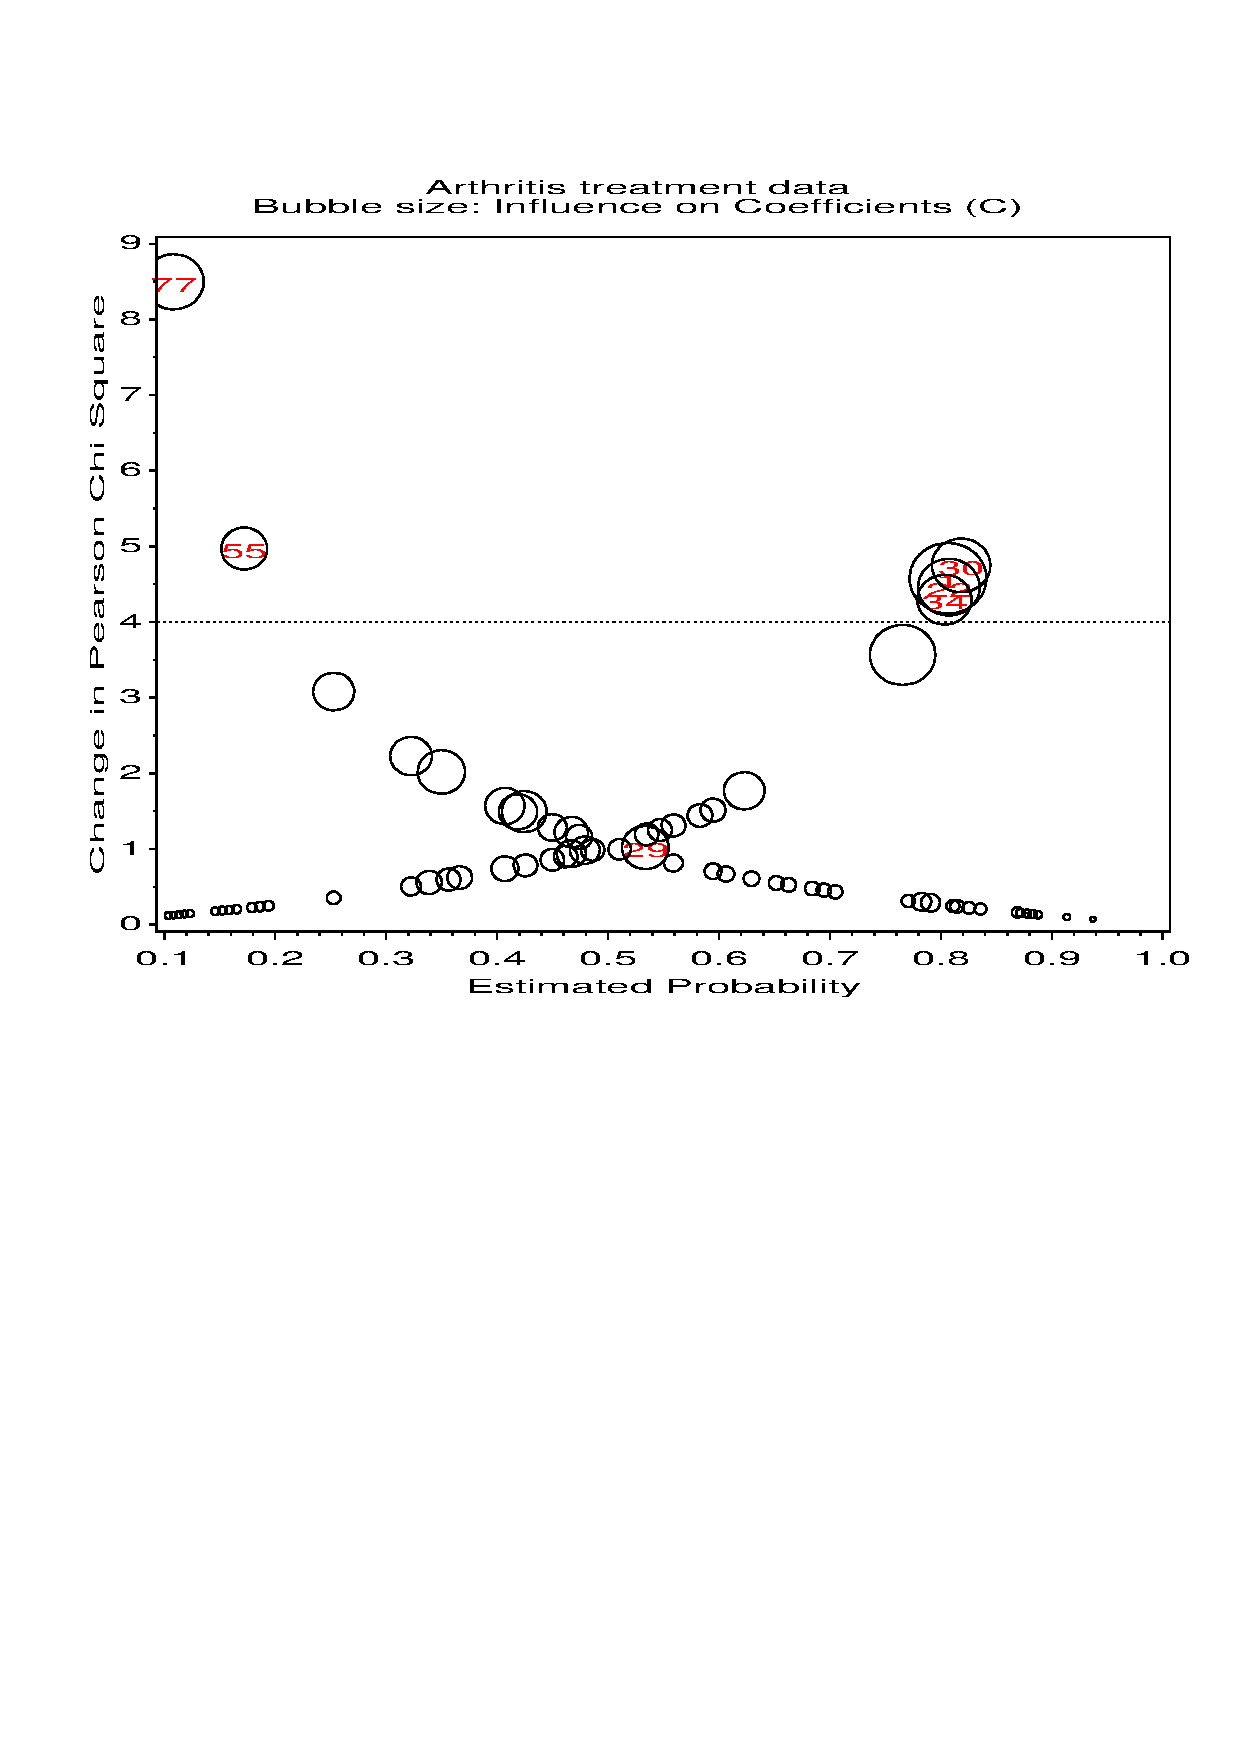
\includegraphics[width=.8\dispwidth,clip]{fig/logist1b1}
 \end{center}

\end{frame}

\begin{frame}
  \frametitle{\macrot{INFLOGIS}: Example}
 \begin{center}
  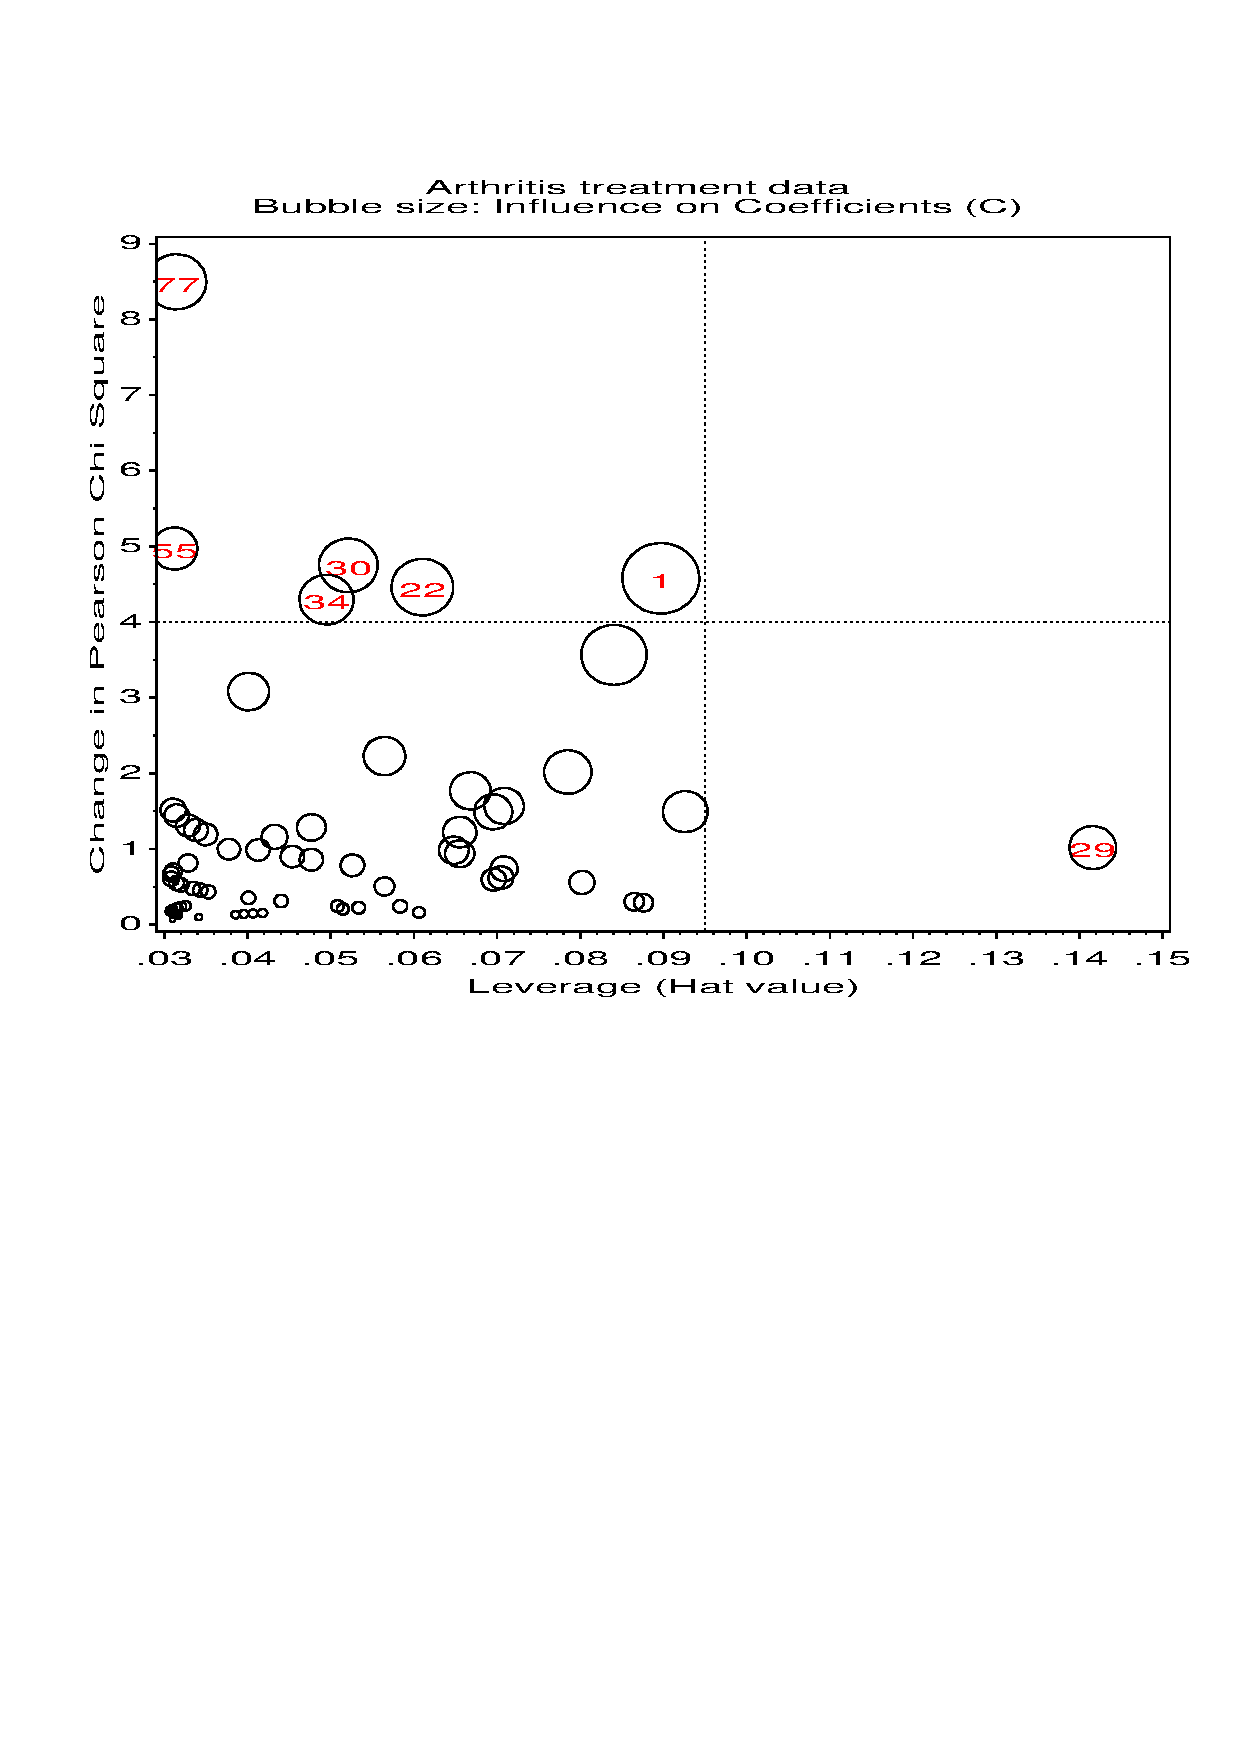
\includegraphics[width=.8\dispwidth,clip]{fig/logist1b2}
 \end{center}

\end{frame}
\subsection{Diagnostic plots in R}
\begin{frame}[fragile]
  \frametitle{Diagnostic plots in R}
In R, plotting a \texttt{glm} object gives the ``regression quartet''
\begin{Rin}[baselinestretch=0.8]
arth.mod1 <- glm(Better ~ Age+Sex+Treatment,data=Arthritis,
             family='binomial')
plot(arth.mod1) 
\end{Rin}

 \begin{center}
  \includegraphics[width=\dispwidth,clip,trim=0 0 0 10]{fig/arthritis-diag1a}
 \end{center}
\end{frame}

\begin{frame}[fragile]
  \frametitle{Diagnostic plots in R}
\begin{Rin}[baselinestretch=0.9]
library(car)
influencePlot(arth.mod1) 
\end{Rin}
 \begin{center}
  \includegraphics[width=.6\dispwidth,clip,trim=0 10 0 10]{fig/arthritis-diag2}
 \end{center}
\end{frame}
